\part{Method}

\chapter{System}
The software that is used in the autonomous landing system is based on the LSTS toolchain \citep{pinto2013lsts}, with \gls{rtk-gps} solution calculated in RTKLib. The toolchain was developed for support of networked heterogeneous air and ocean vehicle systems. The toolchain supports interactions over wireless network, and is supports interaction with different system responseable for the low end control. The toolchain contain four different modules, namely \gls{imc}, DUNE, NEPTUS and Glued.

DUNE (DUNE Uniform Navigation Environment) is a runtime environment for unmanned systems on-board software written in C++. DUNE is capable to interact with sensors, payload and actuators, in addition to communication, navigation, control, manoeuvring, plan execution and vehicle supervision. The software separate operations into different task that each has there own thread of execution. DUNE apply a message bus that is responsible for forwarding \gls{imc} message from the producer to all registered receivers.

Neptus is a Command and Control software which is used to command and monitor unmanned systems that is written in Java. Neptus is able to provide coherent visual interface to command despite the heterogeneity in the controlled system that it is interacting with.  This allow the operator to command and control unmanned system without the need to dwell into specific command and control software in the unmanned system.
\section{Path generation}
The path generator in the  autonomous landing system is designed to enable \gls{uav} landing in both a stationary or moving net. The path is created in two main stages. The first is the creation of the virtual runway, which is defined as a straight line along the heading of the net. The second stage apply a lateral Dubins path \ref{S:DubinsPath} and longitudinal straight line path to create a path that ensures that the \gls{uav} is able to enter the straight line along the virtual runway at the correct height and attitude. The design is inspired by the work done in \citep{Skulstad&Syversen} were way-points was used to guide the \gls{uav} toward the landing approach.

The path parameters are defined through Neptus, which is a command and control software used to create and monitor missions. A Neptus plug-in is used to set and send the path parameters with a IMC message LandingPlanGenerator, which is specificity to create landing paths.

The landing path is design with the assumption that the aerial space in which the \gls{uav} operates is limited.The limitation can be the range of the uav, regulatory limits or weather. In addition the autonomous landing system must be able to perform a safe landing from any initial position. Furthermore the operator must be able to specify the length of the virtual runway, in addition to the decent angle and the construction of the Dubins path.

When the path has been generated the operator can review it in Neptus, such that the operator can determine if the plan should be executed and decide which controllers should be used.  
\subsection{The virtual runway}\label{SS:netApproach}
The virtual runway is inspired by the work done in \citep{Skulstad&Syversen} where waypoint was used to create a straight line path towards the net. This method proved successful, and since the \gls{uav} descent towards the net should be as controlled as possible only small angles is used when transitioning between waypoints. Figure \ref{Fig:LandingPhase} shows the approach towards a stationary net. The landing phase consist of four way-points which is defined relative to the position of the net. The four way-points in the net approach is defined as follows:
\begin{subequations}
\begin{align}
&\mathbf{WP4} = 
\begin{bmatrix}
-a0 \\
0 \\
h_{nc} + a1\tan(\gamma_a) 
\end{bmatrix}\\
&\mathbf{WP3} = 
\begin{bmatrix}
a1 \\
0 \\
h_{nc} - a1\tan(\gamma_a)
\end{bmatrix}\\
&\mathbf{WP2} = \mathbf{WP3} + 
\begin{bmatrix}
a2 \\
0 \\
a2\tan(\gamma_d)
\end{bmatrix}\\
&\mathbf{WP1} = \mathbf{WP2} + 
\begin{bmatrix}
a3 \\
0 \\
0 \\
\end{bmatrix}
\end{align}
\end{subequations}
were the description of the parameters used is given in table \ref{Tb:Approach Parameters}. The net is placed between the first and second way points such that transitional behaviour do not occur during the finale stage of the net landing. In addition the path has been made with the assumption that the $\gamma_a$ and $\gamma_d$ is considered small. This assumption is made to ease the demand of the controllers used in the landing system.
\begin{table}[H]
\begin{center}
    \begin{tabular}{ | l | l |}
    \hline
    \textbf{Parameter} & \textbf{Description} \\ \hline
    $a0$ & The distance behind the net \\ \hline
    $a1$ & The distance in front of the net \\ \hline
    $a2$ & The length of the glide slope \\ \hline
    $a3$ & The length of the approach towards the glide slope \\ \hline
    $\gamma_a$ & The net attack angle \\ \hline
    $\gamma_d$ & The glide slope angle \\ \hline
    \end{tabular}
\end{center}
\caption{Net approach parameters }
\label{Tb:Approach Parameters}
\end{table}
The way point vectors are rotated into the NED frame by a rotation around the z-axes.
\begin{equation}
WP^n = R(\psi_{net})WP^b
\end{equation}
were $\psi_{net}$ is the heading of the net, and $R(\psi_{net})$ is the rotation matrix around the z-axis.
\begin{figure}\label{Fig:LandingPhase}
\def\svgwidth{\textwidth} % Defining the width since Inkscape hasn't done this yet in the .pdf_tex file
\input{InkFig/LandingPhase.pdf_tex}
\end{figure}

\subsection{The landing path approach}\label{SS:LandingApproach}
Before the \gls{uav} can start its decent towards the net it must be at the correct height with correct orientation, which is defined by the length of the run way, in addition to the chosen decent angle. The \gls{uav} should also achive this goal in a controlled manor where the decent it limited to a given decent angle. This is a requirement from any initial position. In addition it's an advantage for the control system if the lateral path is smooth enough for path following purpose.

The lateral path was chosen for the autonomous landing system is Dubins path, due to it's simplicity in description and it fulfils the requirement that it's smooth enough for path following. Since it's desired for the \gls{uav} to decent with small decent angle the longitudinal path is constructed with straight lines. Combined with Dubins path, the circles in the start and end of the path becomes spirals. This increase the demands on the controllers used, since they has to both control the heading in addition to the decent rate with the same control surface. This is the main reason for small angles in the longitudinal path.

The path generation system is designed such that the operator can choose how the path should be generated. The system allows for manual creating of the path, or simply create the shortest path from the start pose to the end pose, which is the first way-point in the path towards the net.
\subsubsection{Shortest path}
When the operator decide that the path should be generated automatically the shortest path from the initial pose to the first way-point is calculated. This is done by calculating all four variants of Dubins path, which is given in table \ref{Tb:DubinsTurningDirection}. After the length of each path is calculated, where the shortest path is chosen to be the landing path.
\subsubsection{Manual path}
If the path should be generated manually the operator has to decide the start and end turning directions.
One mode allow for manual deciding which side the start and finish circle should be in respect on the start pose, and the net landing approach. This allow the operator full control over the landing path, and can choose a landing path that is operation feasible and not necessary the shortest path.
\subsubsection{Longitudinal path}
A desired behaviour in the lateral plane is that the \gls{uav} should have a controlled decent. Given this desired behaviour it was decided that the lateral plane should be a glide slope, which means that the decent angle can be considered small. The strategy chosen to solve this problem is the use of straight lines in the lateral plane. The straight lines are is included with Dubins path such that the turn in Dubins path becomes a spiral.

At the end of Dubins path the path is checked if the correct height has been reach. If the correct height has not been reached the path will create a spiral that converge to the correct height. When the correct height has been reach a last arc is created in order for the \gls{uav} to get the correct orientation.
\subsection{Transition into the net approach}
In order to fully control when the \gls{uav} should start its decent the landing plan can include a loiter at the end of the approach. The loiter manoeuvre can be enabled such that the operator is able to make final preparation with the runway, or used together with a moving net to ease coordination. The loiter manoeuvre is exited when a end manoeuvre signal is sent from Neptus.
\subsection{Plan generation}\label{SS:PlanGeneration}
The plan is configured and generated thought a plug-in in Neptus. In the plug-in the operator can choose how the plan should be generated, as well as the length of the run way and the desired decent rate.
\section{Navigation system}
The navigation system apply \gls{rtk-gps} for position and velocity measurement, which provide higher position accuracy then a standalone \gls{gps}. However the state of the \gls{rtk-gps} can change before or during a mission. Therefore the operator must be able to monitor the state of the \gls{rtk-gps} in Neptus, which is a command and control software used to create and monitor missions. In addition to monitoring the navigation system must be able to handle a drop out of the \gls{rtk-gps}. This is handled in two steps. The first is a short loss compensator stage, where the backup standalone \gls{gps} is compensated to get a position solution closer to the \gls{rtk-gps} solution. The second stage fully disconnect the \gls{rtk-gps}.
\subsection{RTK-GPS system}
The \gls{rtk-gps} solution is calculated in the open-source program liberary RTKLib \citep{takasu2009development}.
The X8 runs the rover program rtkrcv which is connected over TCP/IP with the base station program str2str. Both programs are connected to a Ublox Lea M8T GNSS receiver. The GNSS receiver is programmed to send raw GNSS data to both programs, where the base station program str2str transmits without alteration the raw data to the rover program rtkrcv. The structure of the RTKLib software configured with a rover and base station is shown in figure \ref{figure:RTKLIB_STRUCTURE}.
\clearpage
\begin{figure}[H]
	\centering
		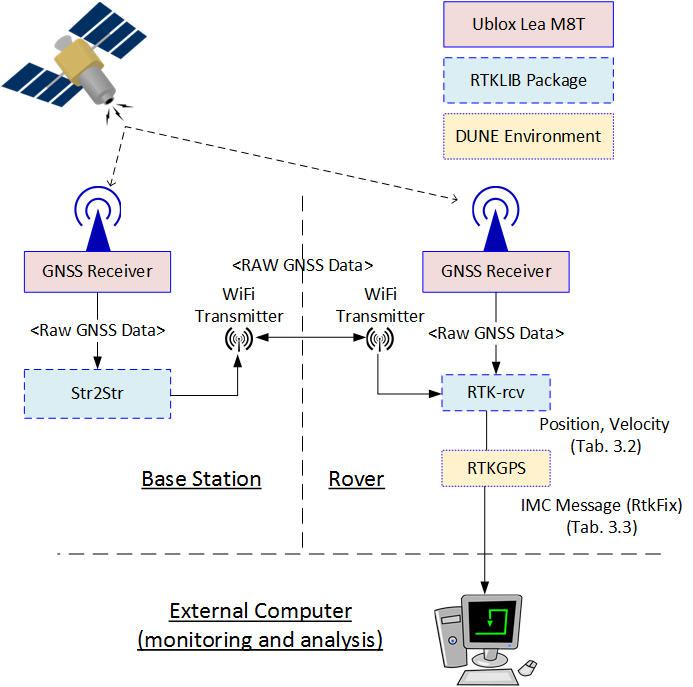
\includegraphics[width=1\textwidth]{figs/RTKLIB.png}
		\caption{The communication structure of \gls{rtklib}}
		\label{figure:RTKLIB_STRUCTURE}
\end{figure}
\clearpage
The navigation system require to now the reference position of the base station in order to use the \gls{rtk-gps} solution. However the base station position is currently not part of the output message from rtkrcv. This is resolved by allowing the base station to calculate it's own position as a standalone \gls{gps}. The \gls{gps} position is transmitted to a local Dune task on the base station, where the operator can decide when the base station can be considered as fixed. When the base station is considered fixed the position is sent to the X8, where it's included in the \gls{rtk-gps} solution message.
\subsection{Navigation state}
The navigation system consists of five states, which is controlled by a state machine. The state transitions is determined by what's available and what the operator has specified should be used. The output from the state machine is the IMC message EstimatedState, which is the only state source used in the Dune control and guidance system. The state machine also dispatch a IMC message that informs which the source used in the navigation system, and which sources is available. Currently only the \gls{rtk-gps} system is considered as a internal system, however this can be expanded to include other sensors used in the Dune system.

The input to the navigation system is IMC message ExternalNav and GpsRtkFix. The ExternalNav message is the primary state source when the \gls{rtk-gps} is not in use, and it's receive the state information from the Pixhawk mounted in the X8.

During a short loss of the \gls{rtk-gps} the position solution in the ExternalNav message is compensated to avoid sudden change in position. The short loss compensator is explain further in \ref{ss:ShortLoss}. The short loss system is implemented to avoid drop out of the \gls{rtk-gps} when a message is delayed, or its struggling due to the dynamic behaviour of the \gls{uav}.

The state machine is depicted in figure \ref{Fig:NavState}, with the edge describtino given in table \ref{Tb:Nav state edge}.

\begin{figure}\label{Fig:NavState}
\def\svgwidth{\textwidth} % Defining the width since Inkscape hasn't done this yet in the .pdf_tex file
\input{InkFig/StateMachine.pdf_tex}
\end{figure}
\begin{table}[H]

    \begin{tabular}{ | p{1cm} | p{8cm} | | p{4cm} |}
    \hline
    \textbf{Edge} 	& \textbf{Event} 										& \textbf{Guard} \\ \hline
    A 				& Event: Received External Nav message 					& None \\ \hline
    B 				& Time out: Fix \gls{rtk-gps} solution for $x$ seconds 	& None \\ \hline
    C 				& Time out: $x$ seconds since last valid GpsFixRtk 		& None \\ \hline
    D 				& Flag: Using Rtk is set true& None \\ \hline
    E 				& Flag: Using Rtk is set false& None \\ \hline
    F 				& Time out: $x$ seconds since last valid GpsFixRtk 		& Short loss compensator:\\ 
      				& Event: Received GpsRtkFix with $type==None$ 			& Enabled\\ \hline
    G 				& Event: Received valid GpsFixRtk message				& None \\ \hline
    H 				& Time out: $x$ seconds since last valid GpsFixRtk 		& Short loss compensator:\\
    				& Event: Received GpsRtkFix with $type==None$			& Disabled \\ \hline
    I 				& Time out: $x$ seconds since last valid GpsFixRtk 		& None \\ \hline
    \end{tabular}

\caption{Net approach parameters }
\label{Tb:Nav state edge}
\end{table}

\subsubsection{Short loss of RTKGPS}\label{ss:ShortLoss}
In the event of \gls{rtk-gps} drop out a offset can be added to the position solution in order to prevent a sudden change in position. The offset is defined as the average difference between the $N$ latest position solution from the \gls{rtk-gps} and the external navigation system:
\begin{equation}
offset = \frac{1}{N}\sum_{n=0}^N(RTKGPS(n)-External(n))
\end{equation}
where the \gls{rtk-gps} solution is displaced into the External nav system. However during the implantation it was discovered that the standard displace function in the DUNE literary was inaccurate in correctly calculating the hight of a offset point. The problem was that the geodetic latitude calculation was calculate assuming that the Earth has a spheric shape. This was solved by creating a new displace function where the geodetic latitude is calculated in according to

%\begin{subequations}
%\begin{align}
%N = \frac{•}{•}
%&\mu = 
%\end{align}
%\end{subequations}

\subsection{Operator interface}
The state of the navigation system is monitored though a interface in Neptus. The interface indicate which source the Dune system is using for state information. The interfaced apply a color code to indicate which source is currently in use in addition to all sensor system that are available, as seen in table \ref{Tb:Color Code}.
\begin{table}[H]
\begin{center}
    \begin{tabular}{ | l | l |}
    \hline
    \textbf{Color} & \textbf{Description} \\ \hline
    White & Not available \\ \hline
    Yellow & Available, but not in use \\ \hline
    Green & Available, and in use \\ \hline
    \end{tabular}
\end{center}
\caption{Net approach parameters }
\label{Tb:Color Code}
\end{table}
\section{Base station}

\section{Guidance and control system system}
The control and guidance system that is used to achive 
The navigation and path generation system is independent of the guidance and control system used in the \gls{uav}. However this section 
The guidance system consist of two part. Sliding mode controller, and a los controller

\subsection{Sliding mode controller}
For course control the system use a sliding mode controller that was proposed in the paper \citep{fortuna2015cascaded}, which USGES stability property.